\subsection{Neural Network Structure}
Neural networks generally have the same constitutive elements, mixed and matched based on the desired performance and complexity of the model that you are trying to build.

\subsubsection{Neural Network Building Blocks}
Generally, neural networks are formed by collections of foundational units, which can generate increasingly complex architectures and yield incredible performance. However, it is always important to start with the fundamental ``atoms'' of the neural network.

The most basic unit of a neural network is the perceptron (or neuron), which is composed of a summation of inputs multiplied by weights, a bias term, and a (typically non-linear) activation function (Fig. \ref{fig:neuron}, Eq. \ref{eq:neuron}). 

\begin{figure}[h!]
    \begin{center}
        {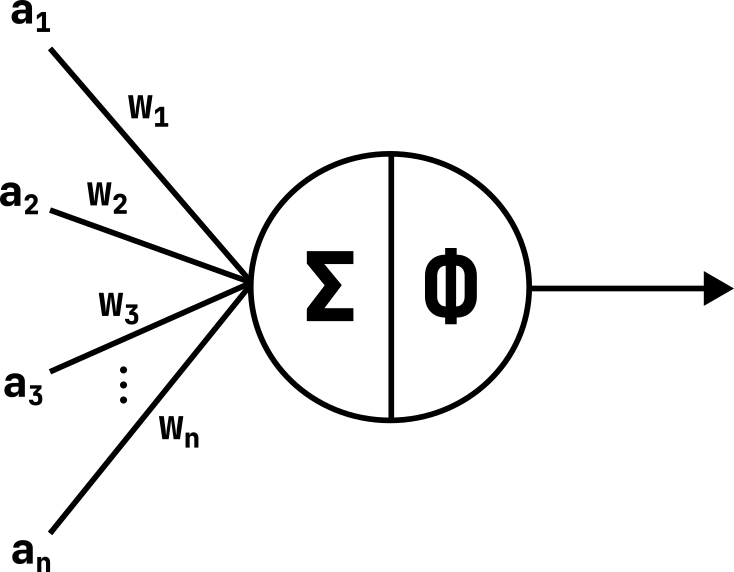
\includegraphics[width=0.55\linewidth]{figs/background/png/neuron.png}}
    \end{center}
    \caption{A schematic representing a single neuron that receives $n$ inputs and applies $\theta$ as an activation function.}
    \label{fig:neuron}
\end{figure}

\begin{equation}
    y = \phi(\sum_{i=1}^{n}a_i w_i + b)
    \label{eq:neuron}
\end{equation}